%% Los cap'itulos inician con \chapter{T'itulo}, estos aparecen numerados y
%% se incluyen en el 'indice general.
%%
%% Recuerda que aqu'i ya puedes escribir acentos como: 'a, 'e, 'i, etc.
%% La letra n con tilde es: 'n.

\chapter{Resultados}

%\section{Estimador Propuesto}

En este capítulo se analizan varias estrategias para la la estimación del parámetro de textura de la distribución $\mathcal{G}_I^0$.
Se ha demostrado que esta distribución es capaz de caracterizar un gran número de objetivos en las imágenes SAR monopolarizada. Está indexada por
tres parámetros: el número de looks (que puede estimarse en toda la imagen), un parámetro de escala, y un parámetro de textura. Este último está estrechamente relacionado con el número
de retrodispersores elementales para cada píxel, esto es una de las razones por las que recibe atención en la literatura. 

Otras de las razones es que el parámetro $\alpha$ de la distribución $\mathcal{G}_I^0$ puede interpretarse en términos de la textura de la imagen. Valores cercanos a $0$, típicamente $\alpha \in [-3,0)$ sugieren zonas extremadamente texturadas como zonas urbanas. Conforme el valor de $\alpha$ decrece indica regiones con moderada textura (usualmente $\alpha \in [-6,-3)$) como son los bosques. Zonas de pastura son compatibles con valores de $\alpha \in (-\infty,-6)$. Esta es otra de las razones por las cuales es muy importante obtener estiamciones precisas de este parámetro.

Entre las técnicas de estimación disponibles, el método de los momentos y el MV estimador son las técnicas clásicas de estimación paramétrica. En~\cite{Bian2013} los autores proponen un método basado en
momentos fraccionarios de bajo orden para estimar la matriz de covarianza en una imagen SAR polarimétrica bajo una distribución alfa estable. En ~\cite{VasconcellosFrerySilva:CompStat,CribariFrerySilva:CSDA} los autores utilizan técnicas de remuestreo para mejorar el rendimiento de estos estimadores en términos de sesgo y error cuadrático medio, a expensas de un alto costo computacional.

Más recientemente~\cite{MellinAnalysisPolSAR,BujorTrouveValetNicolas2004,khan2014} los estimadores basados en la transformada de Mellin, como lo son los LogCumulants y Logmomentos estimadores, han sido implementados con éxito. Tison et al.~\cite{Tison2004} mostraron que los estimadores basados en LogCumulants tienen una mejor performance respecto del MV estimador para el modelo $\mathcal G^0$ para datos de amplitud. Sin embargo estos estimadores no han sido evaluados para el caso de datos de intensidad.

Una propiedad que es deseable que un estimador posea es ser resistente a la presencia de datos atípicos. Bustos et al.~\cite{BustosFreryLucini:Mestimators:2001} y Allende et al.~\cite{AllendeFreryetal:JSCS:05} estudiaron la performance del MV estimador bajo el modelo $\mathcal{G}^{0}$ para datos de amplitud, mostrando que hay una pérdida de robustez ante la presencia de outliers moderados en áreas extremadamente texturadas, mientras que para zonas texturadas la pérdida de robustez ocurre en presencia de outliers severos. Asimismo está falta de robustez es más pronunciada en el caso de muestras de pequeño tamaño. Ellos propusieron como alternativa el M y AM estimador que tienen un buen comportamiento bajo contaminación pero presentan problemas numéricos especialmente para tamaños de muestras chicos.

La idea principal de este trabajo es presentar un nuevo método de estimación para el parámetro de textura del modelo $\mathcal{G}_I^0$ que tenga  buenas propiedades midiéndolas en término de su sesgo, su error cuadrático medior, su capacidad para resistir diferentes niveles de contaminación y de bajo costo computacional. Estas propiedades serán estudiadas incluso para muestras de tamaño pequeño y moderado. Para lograr esta tarea se propone como estimador del parámetro de textura al valor del argumento que minimiza la distancia estocástica entre el modelo teórico y una estimación no paramétrica de la función de densidad subyacente, es decir,
\begin{align}
\widehat{\theta}_n=\mathop{\rm argmin} \limits_{\theta\in\Omega} d(f_{\theta}, \widehat{f}_n)
\end{align}
donde $\Theta$ es el espacio paramétrico y $d$ es una medida de discrepancia, discimilaridad o distancia estocástica, entre la función de densidad teórica $f_{\theta}$ y un estimador no paramétrico $\widehat{f}_n$ de función de densidad teórica.

Esta propuesta está basada en dos pilares: la forma de estimar $\widehat{f}_n$ y la distancia estocástica elegida. En este capítulo daremos argumentos que sugieren que la mejor elección para estimar a la función de densidad subyacente son núcleos asimétricos, señalando que los núcleos Gamma y Lognormal son una buena elección. También sugerimos el método para elegir el ancho de banda, como así también mostraremos que la distancia triangular es una buena medida de discrepancia para este caso.

\subsection{Eligiendo distancias estocásticas}
\label{EligiendoDistancias}

El primer objetivo de este trabajo fue elegir una distancia entre las posibles medidas que ofrece la literatura, para luego elegir el estimador del parámetro de textura a través de la minimización de dicha distancia entre la función de densidad teórica del modelo $\mathcal{G}_I^0$ y una estimación no paramétrica de la función de densidad subyacente. Como se mencionó en el capítulo~\ref{metodologia}, se consideraron las siguientes distancias estocásticas:

\begin{itemize}
	\label{dist}
	\item Distancia de Hellinger $d_\text{\tiny H}(f_\text{\tiny V},f_\text{\tiny W})=1-\displaystyle{\int_{-\infty}^{\infty}\sqrt{f_\text{\tiny V} f_\text{\tiny W}}}$.
	
	\item Distancia de Bhattacharyya $d_\text{\tiny B}(f_\text{\tiny V},f_\text{\tiny W})=-\log\displaystyle{\int_{-\infty}^{\infty}\sqrt{f_\text{\tiny V} f_\text{\tiny W}}}$.
	
	\item Distancia Triangular $d_\text{\tiny T}(f_\text{\tiny V},f_\text{\tiny W}))=\displaystyle{\int_{-\infty}^{\infty}\frac{(f_\text{\tiny V}-f_\text{\tiny W})^2}{f_\text{\tiny V}+f_\text{\tiny W}}}$.
	
	\item Distancia de R\'enyi con parámetro $\beta\in(0,1)$
	$$
	d_\text{\tiny R}^{\beta}(f_\text{\tiny V},f_\text{\tiny W}))=\frac{1}{2(\beta-1)}\log\displaystyle{\int_{-\infty}^{\infty}\big({f_\text{\tiny V}^{\beta}f_\text{\tiny W}^{1-\beta})}+\log\displaystyle{\int_{-\infty}^{\infty}\big(f_\text{\tiny V}^{1-\beta}f_\text{\tiny W}^{\beta}}}\big).
	$$
\end{itemize}
donde V y W son  dos variables aleatorias definidas sobre el mismo espacio de probabilidad cuyas funciones de densidad son $f_\text{\tiny V}(x;\theta_1)$ y $f_\text{\tiny W}(x;\theta_2)$. 
Recordemos que por lo visto en la sección~\ref{MDE} las distancias de Hellinger y Bhattacharyya poseen el mismo mínimo, por este motivo solamente se analizará la distancia de Hellinger.  

Para cumplir con el objetivo inicialmente planteado comenzamos calculando las curvas de distancias entre las funciones de densidad de la distribución $\mathcal G_I^0(\alpha_0, 1-\alpha_0, L)$ y $\mathcal G_I^0(\alpha,1-\alpha,L)$, $\alpha<-1$, para distintos valores de $\alpha_0$ y de $L$. Recordemos que vamos a considerar que el parámtetro de escala cumpla la condición $\gamma^*=-\alpha-1$ para que la $E(Z)=1$ donde $Z \sim \mathcal{G}_I^0(\alpha,\gamma,L)$.

Las figuras~\ref{DistL1},~\ref{DistL3} y~\ref{DistL8} muestran los gráficos, para los casos donde el número de looks $L=\{1,3,8\}$ respectivamente, de las distancias de Hellinger, Rényi y Triangular entre dos distribuciones $\mathcal{G}_I^0$ para valores de $\alpha_0= \{-2,-3,-4,-5,-6,-7\}$. En estos gráficos se puede observar que el comportamiento de las curvas de distancias para los distintos valores de $\alpha_0$ y del número de looks. En todos los casos, cuanto menor es el valor de $\alpha_0$, la curva se hace más plana en un entorno  de él. Esto hace que, al momento de hallar el mínimo, los métodos de optimización sean más inestables y el mínimo sea más difícil de encontrar en forma precisa. Se puede observar también que. a medida que aumenta el valor de $L$, esta situación se revierte y es posible encontrar el mínimo de una forma más eficiente. Recordemos que el número de looks representa la relación señal ruido, por lo tanto, cuanto mayor es el número de looks menor ruido presenta la imagen siendo $L=1$ el caso de mayor ruido. Se puede observar también que la distancia de Hellinger es la que resulta más plana en un entorno del mínimo, y que las distancias de Rényi y Triangular tienen un comportamiento similar.

\begin{figure}[h!]
	\centering    
	\subfigure[Hellinger]{\includegraphics[scale=0.35]{../../Figures/Tesis/Capitulo5/GraficoDHL1_v2.pdf}}
	\subfigure[Rényi]{\includegraphics[scale=0.35]{../../Figures/Tesis/Capitulo5/GraficoDRL1_v2.pdf}}
	\subfigure[Triangular]{\includegraphics[scale=0.35]{../../Figures/Tesis/Capitulo5/GraficoDTL1_v2.pdf}}
	\caption{\label{DistL1}\small L=1}
\end{figure}

\begin{figure}[h!]
	\centering    
	\subfigure[Hellinger]{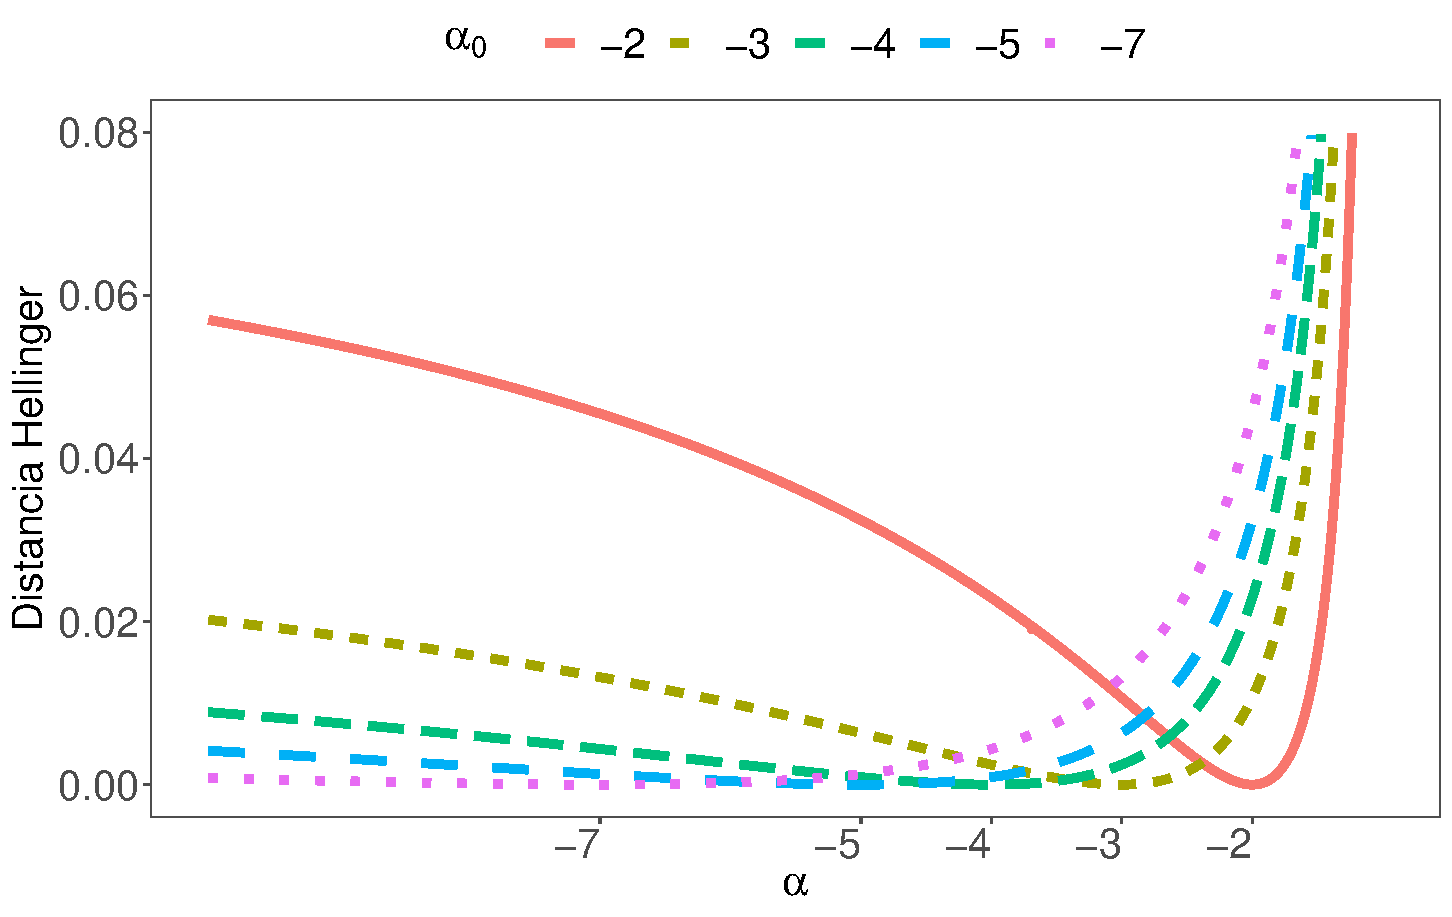
\includegraphics[scale=0.35]{../../Figures/Tesis/Capitulo5/GraficoDHL3_v2.pdf}}
	\subfigure[Rényi]{\includegraphics[scale=0.35]{../../Figures/Tesis/Capitulo5/GraficoDRL3_v2.pdf}}
	\subfigure[Triangular]{\includegraphics[scale=0.35]{../../Figures/Tesis/Capitulo5/GraficoDTL3_v2.pdf}}
	\caption{\label{DistL3}\small L=3}
\end{figure}

\begin{figure}[h!]
	\centering    
	\subfigure[Hellinger]{\includegraphics[scale=0.35]{../../Figures/Tesis/Capitulo5/GraficoDHL8_v2.pdf}}
	\subfigure[Rényi]{\includegraphics[scale=0.35]{../../Figures/Tesis/Capitulo5/GraficoDRL8_v2.pdf}}
	\subfigure[Triangular]{\includegraphics[scale=0.35]{../../Figures/Tesis/Capitulo5/GraficoDTL8_v2.pdf}}
	\caption{\label{DistL8}\small L=8}
\end{figure}

Siguiendo en la búsqueda de la mejor distancia se realizaron simulaciones Montecarlo para elegir la distancia estocástica que mejor performance tiene a la hora de estimar el parámetro de textura de la distribución $\mathcal{G}_I^0$. En Cassetti et al.~\cite{cassettiast2013} se evaluaron dichas distancias pero ahora estimando el parámetro de textura y  comparando la calidad de estos estimadores con el MV estimador en términos del sesgo y del error cuadrático medio. Se realizaron $1000$ replicaciones del experimento que consisten en generar muestras $Z_1, Z_2,\ldots,Z_n$ de variables aleatorias independientes e idénticamente distribuidas donde $Z_i \sim f_{\mathcal{G}_I^0(\alpha,\gamma^*,L)}$ donde el espacio paramétrico está formado por:

\begin{itemize}
	\item Textura: $\alpha=\{-1.5, -3, -5, -8\}$. Con estos valores se describen regiones extramadamente texturadas $(\alpha=-1.5)$, texturadas $(\alpha=\{-3,-5\})$ y homogéneas $(\alpha=-8)$. 
	\item Looks: $L=\{1,3,8\}$, para modelar varios niveles de procesamiento.
	\item Tamaño de muestra: $n=\{9, 25,49, 81,121,1000\}$. 
\end{itemize}

Como se mencionó anteriormente la elección de estos tamaños de muestra se basa en que muchos de los métodos de filtrado de imágenes o detección de bordes utilizan máscaras deslizantes para estimar los parámetros, las cuales suelen ser de tamaño $3 \times 3$,  $5 \times 5$, $7 \times 7$, $9 \times 9$ u  $11 \times 11$. El tamaño de la muestra $n=1000$ se elige para poder estudiar el comportamiento del estimador cuando el tamaño de muestra es grande. 

El valor del parámetro de escala $\gamma^*$ se elige de manera tal que $E(Z)=1$ para que los resultados sean comparables. Esto da una relación entre  $\alpha$ y $\gamma^*$ que es 
\begin{align}
\label{Gama*}
\gamma^*=\alpha-1.
\end{align}
El uso de esta relación nos brinda la posibilidad de llevar un problema de estimación de dos parámetros a estimar un sólo parámetro. 


En cada replicación:
\begin{itemize}
	\item se estima la función de densidad subyacente $\widehat{f}$ utilizando histogramas junto con el método de Freedman Diaconis para elegir el ancho de banda $b$ dado por $b=2 \ \text{IQR}(z_1,\ldots,z_n) n^{-1/3}$ donde $\text{IQR}$ es el rango intercuartil.
	\item se calcula $\widehat{\alpha}= \mathop{\text{argmin}}\limits_{\alpha}d_{\text{D}}(f_{\mathcal{G}_I^0(z,\alpha,1-\alpha,L)},\widehat{f})$ donde D es alguna de las distancias definidas en~\ref{dist}.
\end{itemize} 

De esta manera se obtuvieron $1000$ valores estimados de $\alpha$, $\{\widehat{\alpha}_1, \dots, \widehat{\alpha}_{1000}\}$. Con estos valores se estimó la esperanza, el sesgo y el error cuadrático medio que están definidos por:

\begin{itemize}
	\item $\overline{\widehat{\alpha}}=(1000)^{-1}{\sum_{i=1}^{1000}{\widehat{\alpha}_i}}$
	\item $\widehat{B}(\widehat\alpha) = \overline{\widehat\alpha_i}- \alpha$
	\item $\widehat{\operatorname{\text{ECM}}}=({1000})^{-1}{\sum_{i=1}^{1000}{(\widehat{\alpha}_i-\alpha)^2}}$
\end{itemize}


Las figuras~\ref{ASTalfaL1},~\ref{ASTalfaL2} y~\ref{ASTalfaL3} muestran el sesgo del estimador propuesto para el parámetro de textura $\widehat{\alpha}$ utilizando las distancias de Hellinger, Rényi, Triangular y también Máxima Verosimilitud, para distintos tamaños de muestras $n$ y número de looks $L$. 
La línea recta azul representa el valor verdadero con el que se generaron las muestras. 

En las figuras~\ref{ASTecmL1},~\ref{ASTecmL2} y~\ref{ASTecmL3} se muestra el error cuadrático medio estimado para las mismas combinaciones de parámetros. En este caso la línea azul representa el eje $x$. Los resultados se muestran en escala semilogarítmica para su mejor comprensión visual.
Cabe señalar que la minimización se realizó recorriendo un rango de valores de alfa variando entre $-10$ y $-1$ con paso  $0.1$. 

 
En el gráfico de $L=1$ se observa que para zonas texturadas y homogéneas  $\widehat{\alpha}$ usando distancia triangular tiene un comportamiento similiar al MV estimador en términio de sesgo y ECM. Las distancias de Hellinger y Rényi muestran mayor ECM para tamaños de muestra mayores que $9$, salvo para zonas homogéneas donde el ECM es similar en todas las distancias estudiadas. Asimismo estas distancias muestran un mayor sesgo para muestras grandes.

Para el caso de $L=3$ y $L=8$ vemos que tanto el MV estimador y la distancia triangular siguen manteniendo un comportamiento similar para todos los tipos de zonas consideradas. Incluso, en algunos casos el MDE estimador con esta distancia mejora la performance del MV estimador. Se puede observar que las otras distancias presentan un sesgo y un ECM mayor para zonas texturadas y homogéneas. Asimismo, en estos gráficos se observa que los métodos de minimización de distancias poseen menor error para valores grandes del número de looks. 

\begin{figure}[h!]
	%\centering    
	\subfigure[\small $\widehat{\alpha}$]{\label{ASTalfaL1}\includegraphics[scale=0.4]{../../Figures/Tesis/Capitulo5/ALFAAST_L1.pdf}}
	\subfigure[\small $\widehat{\text{ECM}}$]{\label{ASTecmL1}\includegraphics[scale=0.4]{../../Figures/Tesis/Capitulo5/ECMAST_L1.pdf}}
	\caption{\small L=1}
	\subfigure[\small $\widehat{\alpha}$]{\label{ASTalfaL2}\includegraphics[scale=0.4]{../../Figures/Tesis/Capitulo5/ALFAAST_L3.pdf}}
	\subfigure[\small $\widehat{\text{ECM}}$]{\label{ASTecmL2}\includegraphics[scale=0.4]{../../Figures/Tesis/Capitulo5/ECMAST_L3.pdf}}
	\caption{\small L=3}
	\subfigure[\small $\widehat{\alpha}$]{\label{ASTalfaL3}\includegraphics[scale=0.4]{../../Figures/Tesis/Capitulo5/ALFAAST_L8.pdf}}
	\subfigure[\small $\widehat{\text{ECM}}$]{\label{ASTecmL3}\includegraphics[scale=0.4]{../../Figures/Tesis/Capitulo5/ECMAST_L8.pdf}}
	\caption{\small L=8}
\end{figure}

En Cassetti et al.~\cite{APSAR2013ParameterEstimationStochasticDistances} se aplicó la metodología anterior a una imagen SAR real. En este caso se utilizó una imagen E-SAR~\cite{Horn1996} de un look de los alrededores de Munich. Se utilizó banda L, polarización HH, con $L=1$ en formato intensidad.
E-SAR es un sistema formado por sensores y algoritmos de procesamiento de señales desarrollado, entre otras instituciones, por el centro aeroespacial Deutsches Zentrum für Luft- und Raumfahrt German (DLR), un centro de investigación cuya área principal es la teledetección por microondas.  Principalmente utiliza los sistemas de radar de apertura sintética (SAR), tanto en aire y plataformas aerotransportadas. El compromiso de la institución en los proyectos internacionales ERS-1 y SIR-100 / X-SAR dio origen a los conocidos sistemas aerotransportados SAR y E-SAR. 
%E-SAR opera en las bandas de frecuencia 4, x, C-, L- y P-banda, por lo tanto, cubre un rango de longitudes de onda de 3 a 85 cm. La polarización de la señal de radar es seleccionable, horizontal así como vertical. El modo polarimétrico se conmuta de impulso a impulso en la polarización (HH-HV-W-VH) -secuencia.

En las figuras~\ref{ImagenReales1} y~\ref{ImagenReales1} se muestran dos imágenes E-SAR, de un look, que se utilizaron para testear la performance de las distancias estudiadas y el MV estimador. En ambas figuras se aplicó el método para cada pixel, usando ventanas deslizantes de tamaño $7 \times 7$ y $3 \times 3$ respectivamente. Se puede observar que los resultados son prometedores ya que todas tienen un comportamiento similar y estamos aplicando el método al caso de mayor ruido.


\begin{figure}
	\begin{minipage}[b]{0.45\linewidth} %Una minipágina que cubre la mitad de la página
		\centering
			\centering    
			\subfigure[\label{ImagenReales1} Imagen E-SAR, L=$1$.]{\includegraphics[width=.44\linewidth]{../../Figures/Tesis/Capitulo5/ImHorrible.pdf}}\\
			\subfigure[\label{Real1DH} Hellinger.]{\includegraphics[width=.44\linewidth]{../../Figures/Tesis/Capitulo5/ImHorrible_DH7x7.pdf}}
			\subfigure[\label{Real1DR} R\'enyi, $\beta=0.8$.]{\includegraphics[width=.44\linewidth]{../../Figures/Tesis/Capitulo5/ImHorrible_DR7x7.pdf}}
			\subfigure[\label{Real1DT} Triangular.]{\includegraphics[width=.44\linewidth]{../../Figures/Tesis/Capitulo5/ImHorrible_DT7x7.pdf}}
			\subfigure[\label{Real1MV} MV.]{\includegraphics[width=.44\linewidth]{../../Figures/Tesis/Capitulo5/ImHorrible_MV7x7.pdf}}
			\caption{\small Resultado de estimar el parámetro $\alpha$ para cada pixel, usando ventanas deslizantes de tamaño $7\times 7$.}
	\end{minipage}
\hspace{0.3cm} % Si queremos tener un poco de espacio entre las dos figuras
	\begin{minipage}[b]{0.55\linewidth} %Una minipágina que cubre la mitad de la página
		\centering    
		\subfigure[\label{ImagenReales2} Imagen E-SAR, L=$1$.]{\includegraphics[width=.49\linewidth]{../../Figures/Tesis/Capitulo5/MunichCortadaBien.eps}}\\
		\subfigure[\label{Real2DH} Hellinger.]{\includegraphics[width=.49\linewidth]{../../Figures/Tesis/Capitulo5/MunichCortada3regionesDH.eps}}
		\subfigure[\label{Real2DR} R\'enyi, $\beta=0.8$.]{\includegraphics[width=.49\linewidth]{../../Figures/Tesis/Capitulo5/munichcortada3regionesR.eps}}
		\subfigure[\label{Real2DT} Triangular.]{\includegraphics[width=.49\linewidth]{../../Figures/Tesis/Capitulo5/MunichCortada3regionesDT3x3.eps}}
		\subfigure[\label{Real2MV} MV.]{\includegraphics[width=.49\linewidth]{../../Figures/Tesis/Capitulo5/MunichCortada3RegionesMV.eps}}
		\caption{\small Resultado de estimar el parámetro $\alpha$ para cada pixel, usando ventanas deslizantes de tamaño  $3\times 3$.}
\end{minipage}
\end{figure}
		


Por lo anteriormente expuesto, especialmente por el resulado de las simulaciones, elegimos la distancia Triangular para continuar con el estudio.


\subsection{Incorporando núcleos y evaluando robustez}
\label{jstar}

Como se mencionó en la subsección~\ref{EligiendoDistancias}, en Cassetti et al.~\cite{APSAR2013ParameterEstimationStochasticDistances} se compararon estimadores basados en la distancia de Hellinger, Bhattacharyya, Renyi y Triangular con el MV estimador. Se mostró que la distancia Triangular es la mejor opción para definir el MDE estimador. En ese trabajo se utilizaron histogramas para estimar la función de densidad subyacente $f_S$. En~\cite{gambini2015}, articulo que publicamos en la revista \textit{IEEE Journal of Selected Topics in Applied Earth Observations and
Remote Sensing} se presentaron mejoras con respecto a los resultados obtenidos en~\cite{APSAR2013ParameterEstimationStochasticDistances}: se evalúa el impacto de la contaminación en la estimación de $\widehat{\alpha}$, se emplearon núcleos asimétricos en lugar de histogramas para estimar $f_S$ y se compararon los estimadores basados en la distancia Triangular con el ML estimador, Momentos Fraccionales y LogCumulantes. 

Los estimadores por momentos fraccioneles han sido usado por~\cite{Frery97,GambiniSC08} en el contexto de estimar el parámetro $\alpha$ para datos de amplitud. Para el caso de datos de intensidad, usando la relación $\gamma^*=-\alpha-1$ en~\ref{momento1medio} se tiene que, $\widehat{\alpha}_\text{Mom12}$, el estimador de $\alpha$ usando momentos fraccionales de orden un medio, es el valor de $\alpha$ que resuelve la ecuación:

\begin{equation}
\frac{1}{n} \sum_{i=1}^n \sqrt{Z_i} -\sqrt{\frac{-\widehat\alpha_{\text{Mom12}}-1}{L}}\frac{\Gamma ( -\widehat\alpha_{\text{Mom12}}-{\frac{1}{2}} )}{ \Gamma (-\widehat\alpha_{\text{Mom12}}) }
\frac{\Gamma (L+{\frac{1}{2}} )}{\Gamma (L)}=0.
\label{estim_moment1_2_gI0}
\end{equation}
donde $Z_1,\ldots,Z_n$ es una muestra de variables aleatorias i.i.d proveniente del modelo $\mathcal{G}_I^0$.

En el capítulo~\ref{metodologia} se indicó que $\widehat{\alpha}_\text{ML}$ y $\widehat{\alpha}_\text{LC}$ son soluciones de las ecuaciones~\ref{rootML} y~\ref{eq:logm} respectivamente.

En el modelo modelo multiplicativo para el retorno $Z=X \cdot Y$ con datos monopolarizados presentado en la sección XXX, la variable $Y$ que modela el ruido speckle obedece a una distribución $\Gamma(L,L)$, donde $L$ es el número de looks. La retrodisperción $X$ está modelada por una distribución Inversa Gaussiana Generalizada $\mathcal{N}^{-1}( \alpha ,\lambda ,\gamma )$~\cite{Frery97} donde,  para valores particulares de sus parámetros, se obtienen las distribuciones $\Gamma ( \alpha ,\lambda ) $,  $\Gamma ^{-1}( \alpha ,\gamma ) $ e $IG( \gamma ,\lambda ) $ (Gaussiana Inversa) originando que $Z$ esté modelado por las distribuciones $\mathcal{K}$, $\mathcal{G}_I^{0}$ y $\mathcal{G}^{H}$ respectivamente. La distribución $\mathcal{G}^{H}$ fue propuesta en~\cite{harmoniceusar2000} y describe datos  polarimétricos con bastante precisión, aunque
también se utiliza para imágenes monopolarizadas.

Como se indicó en~\ref{NucleosAsimetricos}, dentro de los núcleos más estudiados se encuentre el núcleo $IG$, $\Gamma$ y Lognormal. En este trabajo~\cite{gambini2015} se estudia la perfomance del núcleo $IG$ para estimar la función de densidad subyacente en el contexto del MDE estimador y se propone como estimador del parámetro de textura del modelo $\mathcal{G}_I^0$ a:

\begin{align}
\widehat{\alpha}_{\text{IG}}= \arg\min_{-20\leq \alpha \leq -1} d_{\text{T}}\big(f_{\mathcal{G}^{0}}(\alpha,\gamma^*, L ), \widehat f_\text{IG}(z)\big),
\label{minimization}
\end{align}
donde $d_{\text{T}}$ es la distancia triangular definida en~\ref{triangular} y $\gamma^*=-\alpha-1$.  

Como es sabido, uno de los puntos importantes en estimación no paramétrica de la función de densidad es el ancho de banda. En esta oportunidad y, a través de estudios empíricos, elegimos un ancho de banda fijo $b=\frac{n^{-1/2}}{5}$.

Ninguno de los problemas planteados para encontrar $\widehat{\alpha}$ tiene una solución explícita, por lo tanto apelamos a procedimientos numéricos acordes a cada estimador, para encontrar dichas soluciones. Un problema común en todos los procedimientos de estimación mencionados anteriormente, incluido ML, y aquellos basados en momentos fraccionales~\cite{Frery97} y LogCumulants~\cite{MellinAnalysisPolSAR,BujorTrouveValetNicolas2004,khan2014} es la necesidad de algoritmos iterativos para los cuales no hay garantía de convergencia a una solución global. Esta falta de convergencia sucede en general, en el caso de muestras de pequeño tamaño. Frery et al.~\cite{FreryCribariSouza:JASP:04} and Pianto and Cribari-Neto~\cite{DealingMonotoneLikelihood} propusieron técnicas que tienen como objetivo aliviar este problema, a expensas de un costo computacional alto.


En la figura~\ref{densidades} se muestra el gráfico de la densidad del modelo $\mathcal{G}_I^0$ para valores de $\alpha=\{-20,-25\}$, $\gamma=\gamma^*$, $L=\{3,8\}$. Se puede observar que estas densidades son muy similares ya que la distribución $\mathcal{G}_I^0$ converge en distribución a una $\Gamma(L,1/L)$ cuando $\alpha \longrightarrow -\infty$. Por este motivo se plantea que $\alpha$ tome valores en el intervalo $[-20,-1]$ en cada método numérico empleado. 

\begin{figure}[h!]
	\subfigure[L=3]{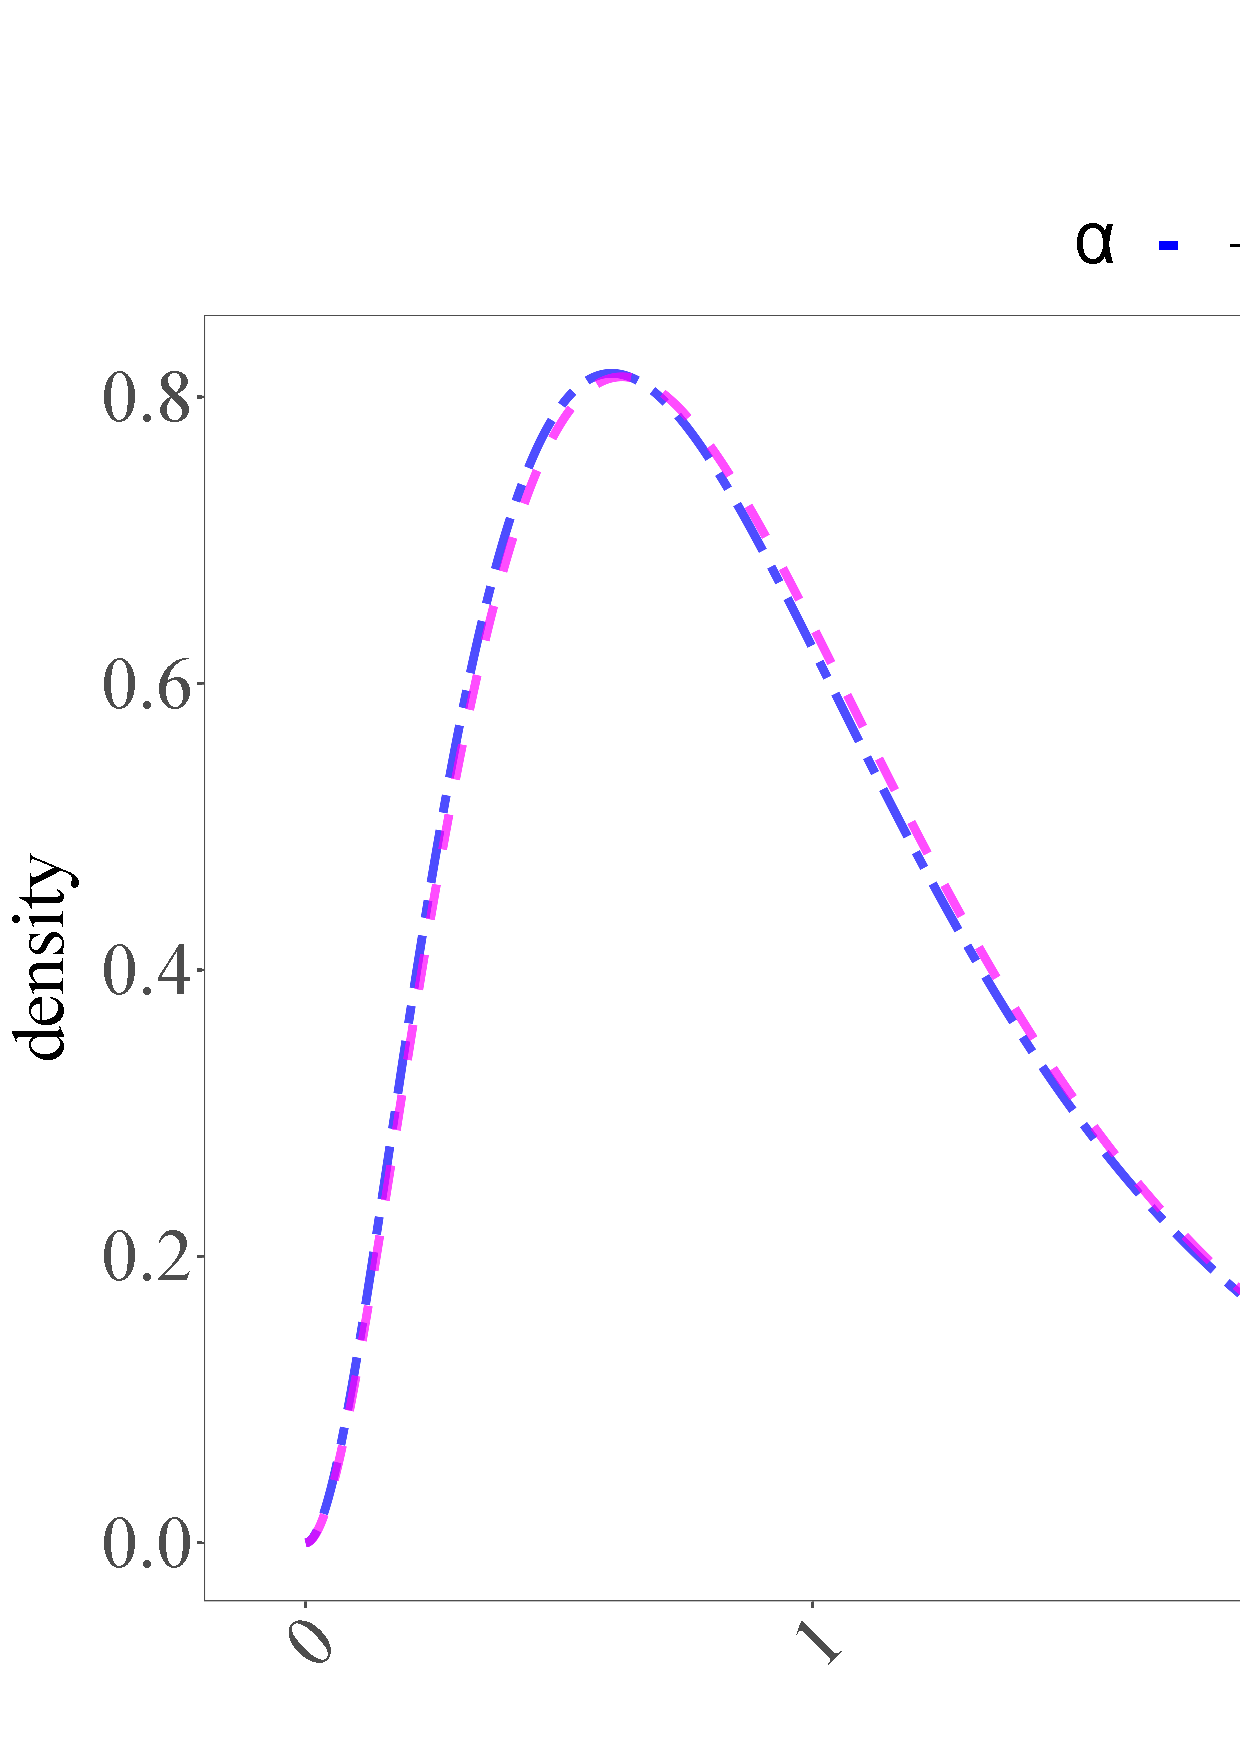
\includegraphics[width=.45\linewidth]{../../Figures/Tesis/Capitulo5/DensidadGI0L3.pdf}}
	\subfigure[L=8]{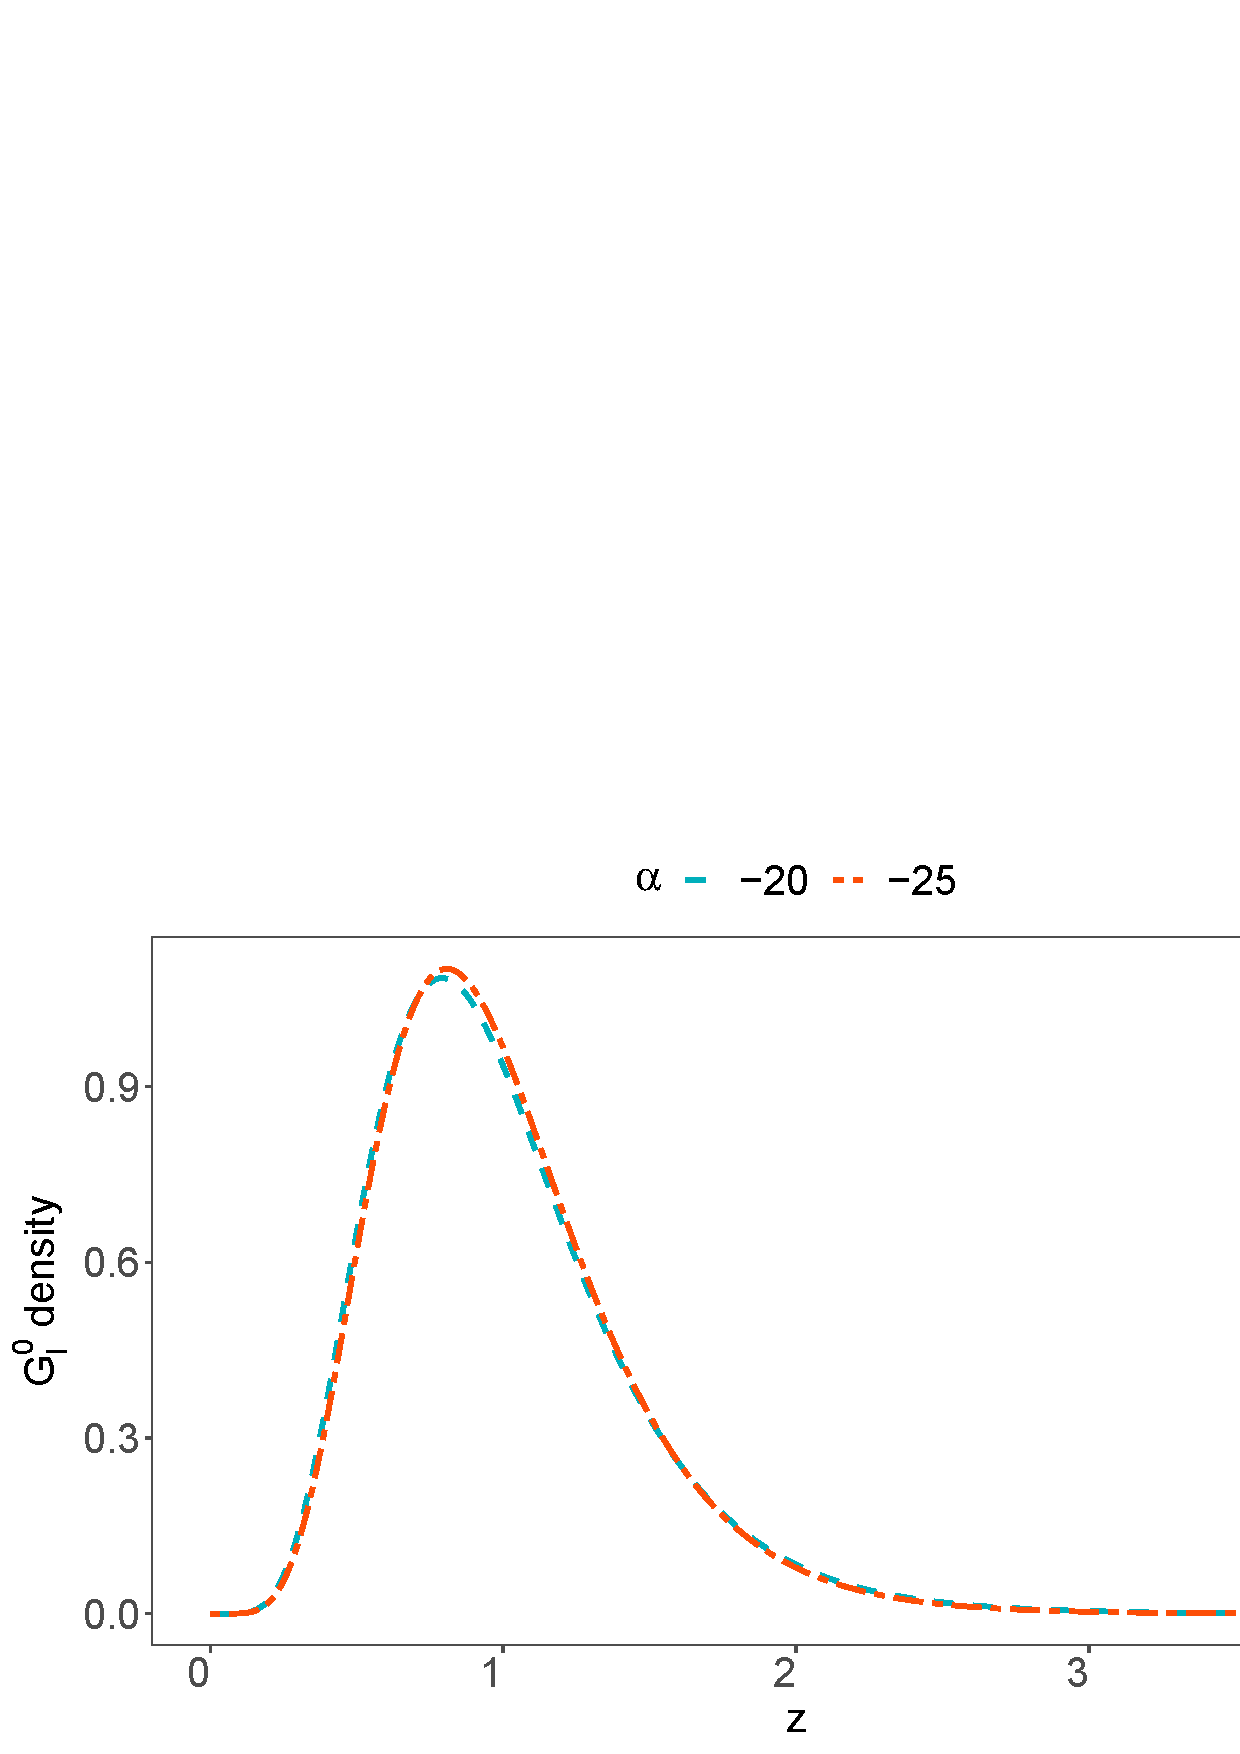
\includegraphics[width=.45\linewidth]{../../Figures/Tesis/Capitulo5/DensidadGI0L8.pdf}}
	\caption{\label{densidades}\small Densidad de $\mathcal{G}_I^0(\alpha,\gamma^*,L)$}
\end{figure}


Se realizó un experimento Monte Carlo para evaluar la performance de cada uno de los estimadores propuestos. El espacio parmétrico consiste en una grilla formada por:
\begin{itemize}
	\item tres valores de textura $\alpha=\{-1.5,-3,-5\}$. Los cuales representan áreas texturadas y extremadamente texturadas.
	\item tres niveles de procesamiento señal-ruido $L=\{1,3,8\}$.
	\item tamaños de muestra $n=\{9,25,49,81,121,1000\}$ compatibles con tamaños de ventana $3,\text{ }5,\text{ }7,\text{ }9$.
\end{itemize}

Se generaron $1000$ muestras para cada punto del espacio paramétrico, y se obtuvieron $\{\widehat{\alpha}_1, \dots, \widehat{\alpha}_{1000}\}$ estimaciones para cada una de estas combinaciones. De esta forma se estimaron la media $\overline{\widehat{\alpha}}=(1000)^{-1}{\sum_{i=1}^{1000}{\widehat{\alpha}_i}}$, el sesgo  $\widehat{B}(\widehat\alpha) = \overline{\widehat\alpha_i}- \alpha$ y el error cuadrático medio $\widehat{\operatorname{mse}}=({1000})^{-1}{\sum_{i=1}^{1000}{(\widehat{\alpha}_i-\alpha)^2}}$ para cada uno de los estimadores estudiados.

En las siguientes figuras ``MV'', ``T'',``Mom12'' and ``LC'' denotarán al estimador basado en el método de Maximum likelihood, distancia Triangular, $\frac{1}{2}$-momento and LogCumulant, respectivamente. En el eje de las abscisas se grafica el tamaño muestral, el cual se presenta en escala semilogarítmica.

Las figuras~\ref{AlfasEstimadosJSTAR2013_L=1},~\ref{AlfasEstimadosJSTAR2013_L=3} y~\ref{AlfasEstimadosJSTAR2013_L=8} muestran la media de $\widehat{\alpha}$ para datos sin contaminar y para diferentes valores de $n$ y $L$. La línea azul representa el verdadero valor de $\alpha$. Se puede observar que solamente dos de los cuatro estimadores se encuentran, en media, muy cercano al verdadero valor: $\widehat{\alpha}_{\text{MV}}$ t $\widehat{\alpha}_{\text{T}}$; es notable el sesgo que presentan  $\widehat{\alpha}_{\text{LC}}$ y $\widehat{\alpha}_{\text{Mom12}}$ para $\alpha=-5$. Se puede observar también que $\widehat\alpha_{\text{ML}}$ tiende a subestimar al verdadero valor de $\alpha$.
Se puede observar que ningún método de estimación tiene el menor error cuadrático medio en todos los casos. El $\widehat{\alpha}_{\text{MOM12}}$ es el que peor se comporta para zonas homogéneas.
%Vasconcellos et al.~\cite{VasconcellosFrerySilva:CompStat} computed a first order approximation of such bias for a closely related model, and our results are in agreement with those.
%The estimator based on the Triangular distance $\widehat\alpha_{\text T}$ compensates this bias.


\begin{figure}[h!]
	\centering
	\subfigure[\label{AlfasEstimadosJSTAR2013_L=1}$\widehat{\alpha}$, L=1]{\includegraphics[width=.47\linewidth]{../../Figures/Tesis/Capitulo5/GraficoAlfaJstar2013_NoCont_L=1.pdf}}
	\subfigure[\label{ECMEstimadosJSTAR2013_L=1}$\widehat{\text{ECM}}$, L=1]{\includegraphics[width=.47\linewidth]{../../Figures/Tesis/Capitulo5/GraficoECMJstar2013_NoCont_L=1.pdf}}
	\subfigure[\label{AlfasEstimadosJSTAR2013_L=3}$\widehat{\alpha}$, L=3]{\includegraphics[width=.47\linewidth]{../../Figures/Tesis/Capitulo5/GraficoAlfaJstar2013_NoCont_L=3.pdf}}
	\subfigure[\label{ECMEstimadosJSTAR2013_L=3}$\widehat{\text{ECM}}$, L=3]{\includegraphics[width=.47\linewidth]{../../Figures/Tesis/Capitulo5/GraficoECMJstar2013_NoCont_L=3.pdf}}
	\subfigure[\label{AlfasEstimadosJSTAR2013_L=8}$\widehat{\alpha}$, L=8]{\includegraphics[width=.47\linewidth]{../../Figures/Tesis/Capitulo5/GraficoAlfaJstar2013_NoCont_L=8.pdf}}
	\subfigure[\label{ECMEstimadosJSTAR2013_L=8}$\widehat{\text{ECM}}$, L=8]{\includegraphics[width=.47\linewidth]{../../Figures/Tesis/Capitulo5/GraficoECMJstar2013_NoCont_L=8.pdf}}
	\caption{\small Datos sin contaminar.}
\end{figure}

%%%%%%%%%%%%%%%%%%%%%%%%%%%%%%%%%%%%%%%%%%%%%%%%%%%%%%%%%% TIEMPO
Se calculó el tiempo medio de procesamiento, medido en segundos, para cada método y cada caso estudiado. Como  ejemplo se presenta, en la tabla~\ref{tablaDeTiemposmedios}, el tiempo medio para $L=1$ and $n=81$. Se puede observar que nuestra propuesta tiene una mayor costo computacional debido a la integración numérica presente en la definición del estimador. Los otros casos son consistentes con los datos de esta tabla. 
Se presentan los detalles de la plataforma informática en el apéndice.

\begin{table}[htb]
	\centering
	\begin{tabular}{cccc}
		\toprule
		MV& DT& Mom$\frac{1}{2}$ & LC \\
		\midrule
		$0.003$& $2.223$ & $0.0001$ &$0.003$ \\
		\bottomrule
	\end{tabular}
\caption{\label{tablaDeTiemposmedios}\small Tiempos medios para datos simulados sin contaminación, $L=1$, $n=81$. }
\end{table}

%%%%%%%%%%%%%%%%%%%%%%%%%%%%%%%%%%%%%%%%%%%%%%%%%%%%%%%%%% ROBUSTEZ
Es muy importante contar con estimadores que sean resistentes a la presencia de datos contaminados, es decir, que sean capaces de producir buenas estimaciones incluso cuando una proporción de los datos no proviene del modelo supuesto como verdadero. Esta situación es de particular importancia en el caso de muestras de pequeño tamaño, por ejemplo, cuando se utilizan filtros que emplean estimadores basados, por lo general, en pequeñas muestras ya que recorren la imagen a través de ventanas deslizantes de tamaño $3 \times 3$, $5 \times 5$ o, por ejemplo, $7 \times 7$. Estas muestras pueden tener datos de zonas con diferentes grado de textura, por ejemplo, en el borde entre diferentes regiones. Esta capacidad de producir buenas estimaciones cuando las observaciones no provienen exactamente del modelo asumido se llama Robustez.

Una de las fuentes de contaminación en las imágenes SAR es el el fenómeno de Double Bounce, donde algunos píxeles tienen un alto valor de retorno. La presencia de tales valores atípicos puede provocar grandes errores en la estimación.

Con el fin de evaluar la robustez de los estimadores, proponemos tres escenarios capaces de describir los desvíos del modelo teórico. Para cada uno de estos escenarios generamos muestras contaminadas donde $0<\epsilon \ll 1$ es la proporción de contaminación. 
Sea  $B$ una variable aleatoria Bernoulli con probabilidad $p$ de ocurrencia de la contaminación. Sea $C \in \mathbb R_+$ un valor grande. Entonces
\begin{itemize}
	\item Caso~1:
	Sean $W$ y $U$ variables aleatorias tales que $W \sim \mathcal{G}_I^0(\alpha_1,\gamma_1^*,L)$, y $U \sim \mathcal{G}_I^0(\alpha_2,\gamma_2^*,L) $. Definimos $Z=BU+(1-B)W$, entonces generamos $\{z_1,\dots,z_n\}$ variables aleatorias independientes, idénticamente distribuidas con función de distribución acumulada dada por:
	$$
	(1-\epsilon) \mathcal{F}_{\mathcal{G}_I^0(\alpha_1,\gamma_1^*,L)}(z)+\epsilon\mathcal{F}_{\mathcal{G}_I^0(\alpha_2,\gamma_2^*,L)}(z),
	$$
	donde $\mathcal{F}_{\mathcal{G}_I^0(\alpha,\gamma,L)}$ es la función de distribución acumulada bajo el modelo $\mathcal{G}_I^0(\alpha,\gamma,L)$.
	%
	\item Case~2: Consideramos $W \sim \mathcal{G}_I^0(\alpha_1,\gamma_1^*,L)$ y el retorno definido como $Z=BC+(1-B)W$.
	\item Case~3:
	Consideramos $W \sim \mathcal{G}_I^0(\alpha,\gamma^*,L)$ y $U\sim \mathcal{G}_I^0(\alpha,10^k\gamma^*,L) $ con $k \in \mathbb{N}$. 
	El retorno $Z=BU+(1-B)W$, entonces $\{z_1,\dots,z_n\}$ son variables aleatorias idénticamente distribuidas con función de distribución acumulada dada por: 
	$$
	(1-\epsilon) \mathcal{F}_{\mathcal{G}_I^0(\alpha,\gamma^*,L)}(z)+\epsilon\mathcal{F}_{\mathcal{G}_I^0(\alpha,10^k\gamma^*,L)}(z).
	$$
\end{itemize}

Todos estos modelos consideran desvíos de la hipótesis del modelo teórico. El primer tipo de contaminación asume que, con probabilidad $\epsilon$, los datos pueden provenir de una distribución perteneciente a la familia de distribuciones $\mathcal{G}_I^0$ pero con otros parámetros. El segundo tipo de contaminación modela, con probabilidad $\epsilon$, un retorno con una valor grande y fijo, digamos $C=100$. El tercer tipo de contaminación es un caso particular del primero, donde la contaminación asume que los datos provienen de una distribución cuyo factor de escala es $k$ órdenes de magnitud mayor que el factor de escala correspondiente al modelo teórico. Analizamos estos tres casos de la contaminación en la evaluación de cada estimador.

%%%%%%%%%%%%%%%%%%%%%%%%%%%%%%%%%%%%%%%%%%%%%%%%%%%%%%%%%%%%%
%%% CASE 1, alpha_2 = -15, epsilon = 0.005

La figura~\ref{Caso1} muestra $\widehat{\alpha}$ y el error cuadrático medio estimado ($\widehat{\text{ECM}}$) para el Caso 1 de contaminación con $\alpha_2=-15$, $\epsilon=0.01$, y variando $n$ y $L$.  
Este tipo de contaminación introduce, con probabilidad $\epsilon=0.01$, observaciones con casi no textura en la muestra bajo análisis. Como se espera, la influencia de tal perturbación es más notable en aquella situaciones donde el modelo subyacente está más alejado de la contaminación. Es decir, para valores grandes de $\alpha$. Esto se ve con claridad en las figuras~\ref{ECMContJSTAR2013Caso1_L=1},\ref{ECMContJSTAR2013Caso1_L=3} y \ref{ECMContJSTAR2013Caso1_L=8} donde el $\widehat{\text{ECM}}$ de $\widehat\alpha_{\text{ML}}$, $\widehat\alpha_{\text{Mom12}}$ y $\widehat\alpha_{\text{LC}}$ son más grandes que el error cuadrático medio de $\widehat\alpha_{\text T}$ para $L=3,8$. Esto no se ve tan claramente para el caso de $L=1$, si se puede decir que $\widehat\alpha_{\text T}$ es competitivo respecto de los otros estimadores para $\alpha=-3,-5$.


\begin{figure}[h!]
	\subfigure[\label{AlfasContJSTAR2013Caso1_L=1}$\widehat{\alpha}$, L=1]{\includegraphics[width=.48\linewidth]{../../Figures/Tesis/Capitulo5/GraficoAlfaJstar2013_Cont_L=1Caso1.pdf}}
	\subfigure[\label{ECMContJSTAR2013Caso1_L=1}$\widehat{\text{ECM}}$ ,L=1]{\includegraphics[width=.48\linewidth]{../../Figures/Tesis/Capitulo5/GraficoECMJstar2013_Cont_L=1Caso1.pdf}}
	\subfigure[\label{AlfasContJSTAR2013Caso1_L=3}$\widehat{\alpha}$, L=3]{\includegraphics[width=.48\linewidth]{../../Figures/Tesis/Capitulo5/GraficoAlfaJstar2013_Cont_L=3Caso1.pdf}}
	\subfigure[\label{ECMContJSTAR2013Caso1_L=3}$\widehat{\text{ECM}}$, L=3]{\includegraphics[width=.48\linewidth]{../../Figures/Tesis/Capitulo5/GraficoECMJstar2013_Cont_L=3Caso1.pdf}}
	\subfigure[\label{AlfasContJSTAR2013Caso1_L=8}$\widehat{\alpha}$, L=8]{\includegraphics[width=.50\linewidth]{../../Figures/Tesis/Capitulo5/GraficoAlfaJstar2013_Cont_L=8Caso1.pdf}}
	\subfigure[\label{ECMContJSTAR2013Caso1_L=8}$\widehat{\text{ECM}}$, L=8]{\includegraphics[width=.50\linewidth]{../../Figures/Tesis/Capitulo5/GraficoECMJstar2013_Cont_L=8Caso1.pdf}}
	\caption{\label{Caso1}\small Datos contaminados: Caso 1, $\epsilon=0.01$.}
\end{figure}

%%%%%%%%%%%%%%%%%%%%%%%%%%%%%%%%%%%%%%%%%%%%%%%%%%%%%%%%%%%%%%%
%%% CASE 2, alpha_2 = -15, epsilon = 0.001, C = 100

La figura~\ref{Caso2} presenta $\widehat{\alpha}$ y $\widehat{\text{ECM}}$ para el Caso 2 de contaminación con $\epsilon=0.001$ y $C=100$. Este tipo de contaminación injecta un valor constante, en este caso $100$, con probabilidad $\epsilon=0.001$. Como estamos considerando muestras con media unitaria, este valor de $C$ respresenta un valor grande de contaminación. En este caso, $\widehat\alpha_{\text T}$ es, en media, más cercano al verdadero valor que los otros métodos, y el valor de $\widehat{\text{ECM}}$ es menor.

\begin{figure}[h!]
	\subfigure[\label{AlfasContJSTAR2013Caso2_L=1}$\widehat{\alpha}$, L=1]{\includegraphics[width=.48\linewidth]{../../Figures/Tesis/Capitulo5/GraficoAlfaJstar2013_Cont_L=1Caso1.pdf}}
	\subfigure[\label{ECMContJSTAR2013Caso2_L=1}$\widehat{\text{ECM}}$ ,L=1]{\includegraphics[width=.48\linewidth]{../../Figures/Tesis/Capitulo5/GraficoECMJstar2013_Cont_L=1Caso1.pdf}}
	\subfigure[\label{AlfasContJSTAR2013Caso2_L=3}$\widehat{\alpha}$, L=3]{\includegraphics[width=.48\linewidth]{../../Figures/Tesis/Capitulo5/GraficoAlfaJstar2013_Cont_L=3Caso1.pdf}}
	\subfigure[\label{ECMContJSTAR2013Caso2_L=3}$\widehat{\text{ECM}}$, L=3]{\includegraphics[width=.48\linewidth]{../../Figures/Tesis/Capitulo5/GraficoECMJstar2013_Cont_L=3Caso1.pdf}}
	\subfigure[\label{AlfasContJSTAR2013Caso2_L=8}$\widehat{\alpha}$, L=8]{\includegraphics[width=.50\linewidth]{../../Figures/Tesis/Capitulo5/GraficoAlfaJstar2013_Cont_L=8Caso1.pdf}}
	\subfigure[\label{ECMContJSTAR2013Caso2_L=8}$\widehat{\text{ECM}}$, L=8]{\includegraphics[width=.50\linewidth]{../../Figures/Tesis/Capitulo5/GraficoECMJstar2013_Cont_L=8Caso1.pdf}}
	\caption{\label{Caso2}\small Datos contaminados: Caso 2, $\epsilon=0.001$.}
\end{figure}

%%% CASE 3, epsilon 0.001, k = 2

La figura~\ref{Caso3} muestra $\widehat{\alpha}$ y $\widehat{\text{ECM}}$ para el Caso 3 de contaminación con $\epsilon=0.005$ y $k=2$. En este caso se contamina la muestra proveniente del modelo verdadero con un observaciones que, con probabilidad $\epsilon=0.005$, provienen de una distribución $\mathcal G_I^0$ con un factor de escala cien veces más grande que el correspondiente al modelo verdadero. El comportamiento de estos estimadores sigue el mismo patrón para $L=3 \text{ y } 8$: $\widehat\alpha_{\text T}$ produce estimaciones más cercanas al verdadero valor con un ECM más chico. No hay un buen estimador para el caso $L=1$ en este caso de contaminación.

\begin{figure}[h!]
	\subfigure[\label{AlfasContJSTAR2013Caso3_L=1}$\widehat{\alpha}$, L=1]{\includegraphics[width=.48\linewidth]{../../Figures/Tesis/Capitulo5/GraficoAlfaJstar2013_Cont_L=1Caso3.pdf}}
	\subfigure[\label{ECMContJSTAR2013Caso3_L=1}$\widehat{\text{ECM}}$ ,L=1]{\includegraphics[width=.48\linewidth]{../../Figures/Tesis/Capitulo5/GraficoECMJstar2013_Cont_L=1Caso3.pdf}}
	\subfigure[\label{AlfasContJSTAR2013Caso3_L=3}$\widehat{\alpha}$, L=3]{\includegraphics[width=.48\linewidth]{../../Figures/Tesis/Capitulo5/GraficoAlfaJstar2013_Cont_L=3Caso3.pdf}}
	\subfigure[\label{ECMContJSTAR2013Caso3_L=3}$\widehat{\text{ECM}}$, L=3]{\includegraphics[width=.48\linewidth]{../../Figures/Tesis/Capitulo5/GraficoECMJstar2013_Cont_L=3Caso3.pdf}}
	\subfigure[\label{AlfasContJSTAR2013Caso3_L=8}$\widehat{\alpha}$, L=8]{\includegraphics[width=.50\linewidth]{../../Figures/Tesis/Capitulo5/GraficoAlfaJstar2013_Cont_L=8Caso3.pdf}}
	\subfigure[\label{ECMContJSTAR2013Caso3_L=8}$\widehat{\text{ECM}}$, L=8]{\includegraphics[width=.50\linewidth]{../../Figures/Tesis/Capitulo5/GraficoECMJstar2013_Cont_L=8Caso3.pdf}}
	\caption{\label{Caso3}\small Datos contaminados: Caso 3, $\epsilon=0.005$.}
\end{figure}

Como se mencionó anteriormente, los algoritmos implementados para los casos de los estimadores Mom12 y LogCumulant no convergen en algunos casos. En el experimento Monte Carlo, si Mom12 o LogCumulant no convergen, eliminamos los estimadores calculados con los otros métodos en esa iteración, por lo que la cantidad de elementos para calcular $\overline{\widehat{\alpha}}$, el sesgo y el error cuadrático medio es menor que $1000$.

La tabla~\ref{tabla_removidos} informa, a modo de ejemplo, el número de casos que fueron removidos para el Caso 1 y $\alpha_2 = -15, \epsilon = 0.01$. Estos resultados son consistentes con los otras escenarios de contaminación, y sugieren que estos métodos son progresivamente más propensos a fallar en áreas más heterogéneas.

\begin{table}[htb]
	\centering
	\begin{tabular}{ccc}
		\toprule
		$L$ & Mom12  & LC \\
		\midrule
		$1$ & $22.87$  & $21.56$ \\
		$3$ & $11.71$  &  $11.87$ \\
		$8$ & $5.81$ & $6.04$  \\
		\bottomrule
	\end{tabular}
\caption{\label{tabla_removidos}Porcentaje de casos de no convergencia para los estimadores de Momentos y LogCumulant en el Caso 1, $\alpha_2 = -15, \epsilon = 0.01$}
\end{table}


%\begin{figure}[h!]
%	\centering
%	\subfigure[\label{AlfasContJSTAR2013Caso1_L=1}$\widehat{\alpha}$]{\includegraphics[width=.48\linewidth]{../../Figures/Tesis/Capitulo5/GraficoAlfaJstar2013_Cont_L=1Caso1.pdf}}
%	\subfigure[\label{ECMContJSTAR2013Caso1_L=1}ECM]{\includegraphics[width=.48\linewidth]{../../Figures/Tesis/Capitulo5/GraficoECMJstar2013_Cont_L=1Caso1.pdf}}
%	\caption{\small Datos contaminados: Caso1, L=1.}
%\end{figure}
%
%\begin{figure}[h!]
%	\centering
%	\subfigure[\label{AlfasContJSTAR2013Caso1_L=3}$\widehat{\alpha}$]{\includegraphics[width=.47\linewidth]{../../Figures/Tesis/Capitulo5/GraficoAlfaJstar2013_Cont_L=3Caso1.pdf}}
%	\subfigure[\label{ECMContJSTAR2013Caso1_L=3}ECM]{\includegraphics[width=.47\linewidth]{../../Figures/Tesis/Capitulo5/GraficoECMJstar2013_Cont_L=3Caso1.pdf}}
%	\caption{\small Datos contaminados: Caso1, L=3.}
%\end{figure}
%
%\begin{figure}[h!]
%	\centering
%	\subfigure[\label{AlfasContJSTAR2013Caso1_L=8}$\widehat{\alpha}$]{\includegraphics[width=.47\linewidth]{../../Figures/Tesis/Capitulo5/GraficoAlfaJstar2013_Cont_L=8Caso1.pdf}}
%	\subfigure[\label{ECMContJSTAR2013Caso1_L=8}ECM]{\includegraphics[width=.47\linewidth]{../../Figures/Tesis/Capitulo5/GraficoECMJstar2013_Cont_L=8Caso1.pdf}}
%	\caption{\small Datos contaminados: Caso1, L=8.}
%\end{figure}
%\begin{figure}[h!]
%	\centering
%	\subfigure[\label{AlfasEstimadosJSTAR2013_L=3}$\widehat{\alpha}$]{\includegraphics[width=.47\linewidth]{../../Figures/Tesis/Capitulo5/GraficoAlfaJstar2013NoContL=3.pdf}}
%	\subfigure[\label{ECMEstimadosJSTAR2013_L=3}ECM]{\includegraphics[width=.47\linewidth]{../../Figures/Tesis/Capitulo5/GraficoECMJstar2013NoContL=3.pdf}}
%	\caption{\small  Datos sin contaminar, L=3.}
%\end{figure}
%
%\begin{figure}[h!]
%	\subfigure[\label{AlfasEstimadosJSTAR2013_L=8}$\widehat{\alpha}$]{\includegraphics[width=.47\linewidth]{../../Figures/Tesis/Capitulo5/GraficoAlfaJstar2013NoContL=8.pdf}}
%	\subfigure[\label{ECMEstimadosJSTAR2013_L=8}ECM]{\includegraphics[width=.47\linewidth]{../../Figures/Tesis/Capitulo5/GraficoECMJstar2013NoContL=8.pdf}}
%	\caption{\small Datos sin contaminar, L=8.}
%\end{figure}

Hemos aplicado estos métodos en una imagen real, la misma imagen utilizada en Cassetti et al.~\cite{APSAR2013ParameterEstimationStochasticDistances}, una imagen E-SAR~\cite{Horn1996} de un look de los alrededores de Munich, banda L, polarización HH en formato intensidad. La figura~\ref{reales2} muestra las regiones usadas para estimar el parámetro de textura. Esta imagen tiene $300\times250$ pixels y comprende principalmente dos áreas de cultivo diferentes.

\begin{figure}[hbt]
	\centering
	\includegraphics[width=.52\linewidth,angle=-90]{../../Figures/Tesis/Capitulo5/MunchCortadaReg.pdf}
	\caption{\label{reales2}Image real E-SAR junto con la regiones usadas para estimar el parámetro $\alpha$.}
\end{figure}

La tabla~\ref{tablaResultadosMunich} muestra los resultados de las estimaciones del parámetro $\alpha$ para cada región rectangular junto con los tiempos de procesamiento, donde $NA$ significa que no fue posible estimar el correspondiente estimador ya que el algoritmo no convergió. 

\begin{table}[htb]
	\centering
	\begin{tabular}{c*9{c}}
		\toprule
		\multirow{2 }{*} {Color} & \multirow{2 }{*}{n} & \multirow{2 }{*}{$\widehat{\alpha}_{\text MV}$} & \multirow{2 }{*}{$\widehat\alpha_{\text T}$} & \multirow{2 }{*}{$\widehat\alpha_{\text{Mom12}}$} & \multirow{2 }{*}{$\widehat\alpha_{\text{LC}}$} & \small Tiempo  &  \small Tiempo & \small Tiempo &  \small Tiempo  \\
		&      &                        &                           &                                 &                                &  \small MV &  \small DT &   \small Mom12 &  LC \\
		\midrule
		Magenta   & $100$  & $-1.9$ & $-2.7$ & $-1.9$  & $-1.7$  & $0.03$ & $5.85$ & $0.03$  & $0.02$\\
		Amarillo  & $90$   & $-6.2$ & $-5.1$ & $-6.6$  & $-6.8$  & $0.00$ &$5.16$  & $0.00$  & $0.00$\\
		Rojo      & $64$   & $-1.8$ & $-1.9$ & $-1.9$  & $-1.8$  & $ 0.00 $&$4.17$ & $0.00$  & $0.00$\\
		Verde     & $48$   & $-2.5$ & $-2.5$ & $-2.9$  & $-3.1$  & $0.00$ & $3.31$ & $ 0.00$ & $0.00$\\
		Azul      & $25$   & $-4.9$ & $-3.0$ &  $NA$   & $NA$    & $0.00$ & $2.08$ & $0.00$  & $0.00$\\
		\bottomrule
	\end{tabular}
\caption{\label{tablaResultadosMunich}$\widehat{\alpha}$ para las muestras de la figura~\ref{reales2}}
\end{table}

Aplicamos el test de Kolmogorov-Smirnov (KS-test) como otra estrategia para evaluar a los estimadores bajo estudio. Se aplicó el test a dos muestras: una muestra $\bm x$ que proviene de la imagen, y una segunda muestra $\bm y$ simulada.
Babu and Feigelson~\cite{Jogesh2006} alertan sobre el uso de la misma muestra para estimar los parámetros y para realizar el KS test, porque se pueden sacar conclusiones erróneas. Entonces tomamos una muestra de la imagen real $\bm x$ usada para estimar los parámetros con los cuatro métodos bajo análisis y la comparamos con una muestra simulada $\bm y$, del mismo tamaño, proveniente de una distribución $\mathcal G_I^0$ con los parámetros estimados. Se aplicó el KS test entre $\bm x$ y $\bm y$ considerando la hipótesis nula $H_0$ ``ambas muestras provienen de la misma distribución'', y el complemento de esta hipótesis como hipótesis alternativa.

Table~\ref{resultadosTestMunich} muestra los $p$-valores. Se puede observar que no hay suficiente evidencia para rechazar la hipótesis nula con un nivel de signficación del $5$\% en cualquiera de los casos.
%This result justifies the adequacy of the model for the data.
%Se aplica  el test de Kolmogorov Smirnov utilizando dos muestras de datos $X$ e $Y$. La muestra $X$ proviene de la imagen real (cuyo número equivalente de looks $L$ es conocido), de tamaño $n$. Luego se estima el parámetro $\hat{\alpha}$ utilizando esta muestra. Luego se genera una muestra simulada $Y$ con distribución $\mathcal{G}^0_I(\hat{\alpha},n,L)$ y se calcula el test de hipótesis $K-S$ con la hipótesis nula $H_0= \text{Ambas muestras poseen la misma distribución}$ y $H_A= \text{Las muestras no poseen la misma distribución}$. La siguiente tambla muestra los resultados de los p-valores obtenidos. Se observa que no se rechaza la hipótesis nula en ninguno de los casos.

\begin{table*}[htb]
	\caption{ $p$-valor del KS test para las muestras de la imagen de la figura~\ref{reales2}  }
	\centering
	\begin{tabular}{c*4{c}}
		\toprule
		Color      & TestMV    & TestDT    & TestMom12  &TestLC \\
		\midrule
		Magenta    & $0.46$    & $ 0.58$   & $0.28$   & $0.69$\\
		Amarillo   & $0.63$    & $0.98$    & $0.76$  & $0.22$\\
		Rojo       & $0.30$    & $ 0.30$   & $0.21$   & $0.99$\\
		Verde      & $0.37$    & $0.85$    & $0.37$   & $0.37$\\
		Azul       & $0.15$    & $0.07$    & $NA $    & $NA $\\
		\bottomrule
	\end{tabular}
	\label{resultadosTestMunich}
\end{table*}

La figura~\ref{reales3} muestra las regiones usadas para estimar el parámetro de textura bajo la influencia de un corner reflector. 
La tabla~\ref{resultadosCorner} muestra los valores de  $\widehat{\alpha}$ para cada área rectangular en la imagen de la figura~\ref{Cornerregiones}.

Los estimadores MV, Mom12 y LogCumulant son incapaces de producir una estimación en pequeñas muestras.  Se puede observar que tanto $\widehat\alpha_{\text{Mom12}}$ como $\widehat\alpha_{\text{LC}}$ requieren al menos un tamaño de muestra de $90$ observaciones para que se pueda dar una estimación para $\alpha$. El estimador basado en la distancia triangular produce valores plausibles bajo contaminación incluso con muestras muy pequeñas.

\begin{figure}[htb]
	\centering
	\subfigure[Single-look E-SAR imagen con un corner reflector.]{\includegraphics[angle =90,width=.8\linewidth]{../../Figures/Tesis/Capitulo5/Corner.pdf}}
	\subfigure[\label{Cornerregiones} Regiones de interés.]{\includegraphics[angle =90,width=.8\linewidth,]{../../Figures/Tesis/Capitulo5/CornerReg}}
	\caption{\label{reales3} $\widehat{\alpha}$ estimado con muestras de varios tamaños en una imagen real SAR con un corner reflector.}
\end{figure}



\begin{table*}[htb]
	\centering
	\caption{$\widehat{\alpha}$ y tiempos de procesos para las muestras mostradas en la figura~\ref{Cornerregiones}}
	\label{resultadosCorner}
	\begin{tabular}{c*9{c}}
	\toprule
	\multirow{2 }{*} {Color} & \multirow{2 }{*}{n} & \multirow{2 }{*}{$\widehat\alpha_{\text MV}$} & \multirow{2 }{*}{$\widehat\alpha_{\text T}$} & \multirow{2 }{*}{$\widehat\alpha_{\text{Mom12}}$} & \multirow{2 }{*}{$\widehat\alpha_{\text{LC}}$} & \small Tiempo  &  \small Tiempo & \small Tiempo &  \small Tiempo  \\
	&      &                        &                           &                                 &                                &  \small MV &  \small DT &   \small Mom12 &  LC \\
	\midrule
		Magenta     & $15$  & $-20.0$ & $-4.1$  & $NA $   & $NA $     &  $0.03$  &  $ 1.95 $    &  $ 0.03$   &  $0.03$ \\
		Verde       & $42$  & $-9.2$  & $-5.0$  & $NA$    & $ NA $    &  $0.00$  &  $ 4.04$     &  $ 0.00$   &  $ 0.00$\\
		Azul        & $90$  & $-3.5$  & $-2.7$  & $-4.7$  & $-14.2$   &  $0.02$  &  $4.85$      &  $ 0.00$   &  $0.00$\\
		Amarillo    & $156$ & $-2.2$  & $-1.8$  & $-2.6$  & $-3.4$    &  $0.01$  &  $8.35$      &  $0.00$    &  $0.00$\\
		Rojo        & $225$ & $-1.9 $ & $-1.7$  & $-2.1$  & $ -2.5 $  &  $0.02$  & $ 10.97$     &  $ 0.00$   &  $0.00$\\
		\bottomrule
	\end{tabular}
\end{table*}

La tabla~\ref{pvaluesTrueNestedSamples} presenta los $p$-valores del KS test aplicado, como se indicó anteriormente, a las muestras señaladas en la figura~\ref{Cornerregiones}

Como se mencionó anteriormente el $\widehat\alpha_{\text{Mom12}}$ y $\widehat\alpha_{\text{LC}}$ no pudieron producir estimaciones en dos muestras y, por lo tanto, no fue posible aplicar el test. En el único caso donde se rechaza la hipótesis nula: las muestras provienen de la misma distribución, es para la muestra azul y el MV estimador. 

Estos resultados nos llevan a concluir que el modelo $\mathcal{G}_I^0$ es una buena opción para modelar adecuadamente datos provenientes de imágenes SAR con datos de intensidad ante la presencia de contaminación. Asimismo podemos concluir que el estimador propuesto es una buena elección para estimar el parámetro de textura de la distribución $\mathcal{G}_I^0$, ya que es competitivo frente al MV estimador y mejora a los otros dos estimadores estudiados especialmente para el caso de muestras de pequeño tamaño.

\begin{table*}[htb]
	\centering
	\caption{$p$-valores del KS test para la muestras indicadas en la figura~\ref{Cornerregiones}}
	\label{pvaluesTrueNestedSamples}
	\begin{tabular}{c*4{r}}
		\toprule
		Color       &  TestMV    &  TestDT    &  TestMom12  &  TestLC\\
		\midrule
		Magenta     & $ 0.38$    & $ 0.93 $   & $ NA $     & $  NA$\\
		Green       & $ 0.11$    & $ 0.93$    & $ NA $     & $   NA$\\
		Blue        & $ 0.01 $   & $0.11 $    & $ 0.40$    & $ 0.11$\\
		Yellow      & $0.19$     & $0.31$     & $ 0.46 $   & $0.15$\\
		Red         & $0.23$     & $0.12$     & $ 0.008$   & $0.02$\\
		\bottomrule
	\end{tabular}
\end{table*}
%\begin{table}[hbt]
%	\centering
%	\caption{Número de casos de no convergencia para distancia triangular generalizada, L=$3$}
%	\label{NoConvDTG}
%		\begin{tabular}{c*7{r}}
%			\toprule		
%			$\alpha$ & $n$ & s=$1$ & s=$1.5$ & s=$2$ & s=$3$ & s=$4$\\
%			\midrule
%			\multirow{3 }{*}{$-1.5$} 
%			& $9$  & $26$ & $14$ & $11$ & $7$ & $6$ \\ 
%			& $25$ & $0 $ & $0 $ & $0$  & $0$ & $0$\\ 
%			& $49$ & $0$  & $1 $ & $1$  & $0$ & $0$\\ 
%			\midrule
%			\multirow{3 }{*}{$-3$}
%			& $9$  & $10$ & $6 $ & $5$  & $4$ & $4$ \\ 
%			& $25$ & $0$  & $1 $ & $1$  & $1$ & $0$\\ 
%			& $49$ & $0$  & $0$  & $0$  & $0$ & $0$\\ 
%			\midrule
%			\multirow{3 }{*}{$-5$} 
%			& $9$  & $4 $ & $3 $ & $3$  & $2$ & $1$\\ 
%			& $25$ & $1 $ & $1 $ & $1$  & $0$ & $0$\\ 
%			& $49$ & $0$  & $0 $ & $0$  & $0$ & $0$\\ 
%			\midrule
%			\multirow{3 }{*}{$-8$} 
%			& $0$ & $0$ & $0$ & $0$  & $0$ & $0$\\ 
%			& $0$ & $0$ & $0$ & $0$  & $0$ & $0$\\ 
%			& $0$ & $0$ & $0$ & $0$  & $0$ & $0$\\ 
%			\midrule
%			\bottomrule 	
%		\end{tabular}
%\end{table}	

\subsection{Mejorando la propuesta}
\label{mejorando}

\subsection{Resultados teóricos}